%%%%%%%%%%%%%%%%%%%%%%%%%%%%%%%%%%%%%%%%%%%%%%%%%
%                                               %
%filename	mm.tex				%
%author		wakemecn			%
%date		6/23/2011			%
%                                               %
%%%%%%%%%%%%%%%%%%%%%%%%%%%%%%%%%%%%%%%%%%%%%%%%%

%\documentclass{article}
%\usepackage{xeCJK}
%\setmainfont[BoldFont=SimHei]{SimSun%}
%\setmonofont{SimSun}
%\XeTeXlinebreaklocale"zh"
%\begin{document}
\subsection{内存管理模块}
		模块从系统预先申请256B,512B,1KB,2KB,$\ldots$,$2^n$KB等2幂次大小的块
		各若干。通过mem\_chunk结构维护特定大小的内存块大小的幂级,预分配的数目,
		已被使用的块链表和空闲的块链表。指针数组维护所有大小块的mem\_chuck结构
		指针。当申请使用M KB($2^m < M < 2^n$)空间时,若$2^n$KB大小块仍有空
		闲块,则将其分配,并将该块移动至已使用块链表中;若上述大小的块不存
		在空闲块或者不存在该大小的块,则模块动态申请若干数目该大小块的内存区域,
		分配内存。当释放某大小块时,若检测到释放的块位于模块动态申请的内存中
		时,则释放该内存。
\begin{figure}[H]
\centering
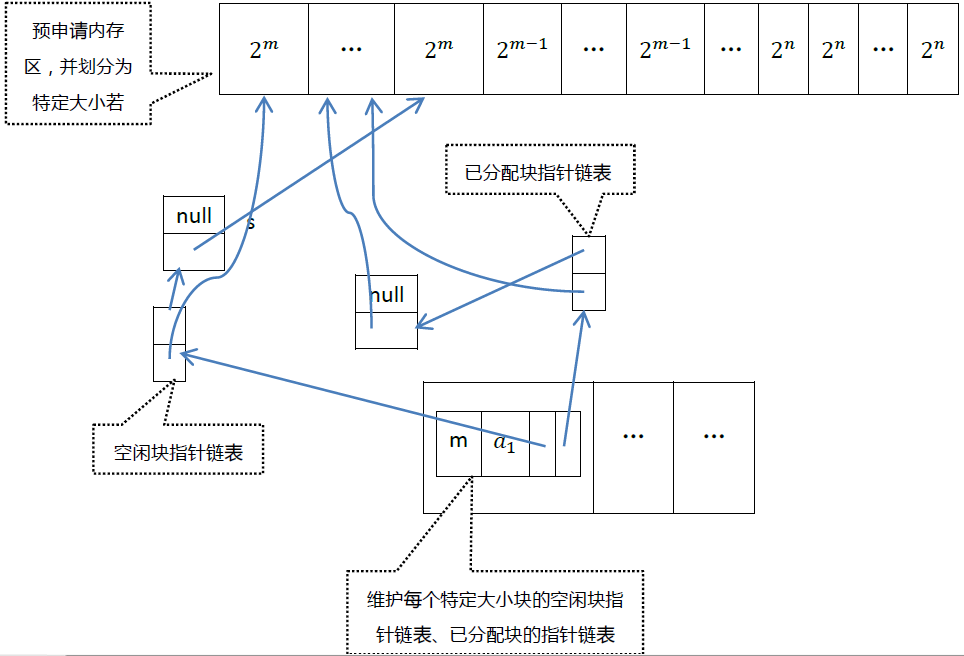
\includegraphics[keepaspectratio,scale=0.5]{pitures/mm.png}
\caption{内存管理示意图}
\end{figure}


%%%%%%%%%%%%%%%%	end of mm.tex    %%%%%%%%%%%%%%%
